\section{公司}
\subsection{公司名称}
一课,缩写为ike(Internet Knowledge and Experience)。知识改变命运。
\subsection{公司简介}
\subsubsection{公司性质}\

有限责任公司
\subsubsection{公司理念}\

核心价值观是企业文化的灵魂,是企业的特质,是行动的准则,也是我们共同的信念。它使企业有了互信互谅的工作氛围,使企业有了创新变革的前进勇气,使企业有了合作共赢的奋斗理想,使企业有了争做第一的远景展望。我们创业团队的核心价值观就是:善于学习,勇于创新,团结协作,服务大众。

本公司将把核心价值观渗透到公司的日常管理中,使以企业核心价值观为中心的企业文化成为每个人坚定的信念,使企业核心价值观贯彻在每个人的一言一行、一举一动中,使核心价值观溶化在每一个人的血液里,使企业核心价值观体现在战略思考、战略执行的结果中,这将是我们始终如一的信念。

\subsubsection{公司目标}\

本公司将持续不断的健全管理机制,培育核心技术能力,建立竞争优势,增强自我完善和自我发展的能力;同时我们会履行社会责任,服务于社会、回报于社会,为整个价值链系统创造最大的价值;专心专意打造一流的在线教育平台,为产业创新的良性发展注入成功基因,整合优势的资源,为国家的进步、社会的创新做贡献。行为识别是企业识别系统(CIS)中的重要方面,是企业理念付诸于计划行为的方式。它是企业员工如何履行职责的行为规范。它在组织制度、管理培训、行为规则、公关礼仪等方面表现出来,使抽象的理念化为有形的行为,是我们在实际行动中的目标。在企业识别系统(CIS)中,行为识别有着最广泛的内容,这也是我们公司所期待达成的目标:
\paragraph{企业员工共同行为规范:}\

关心政治,善于学习 热爱企业,忠于职守

发扬传统,勇于创新 钻研业务,讲求效率

团结协作,遵章守纪 艰苦奋斗,厉行节约

\paragraph{企业管理人员行为规范:}\

政治坚定,诚信经营 发扬传统,勇于创新

科学管理,民主决策 维护团结,作风正派

勤俭节约,廉洁奉公 关心职工,联系群众

\subsection{公司控股结构}
%还没写啊!!!!!!!!!!!!!!!!!!!!!!!!!

\subsection{公司架构}
公司架构:
\begin{figure}[H]
	\centering
	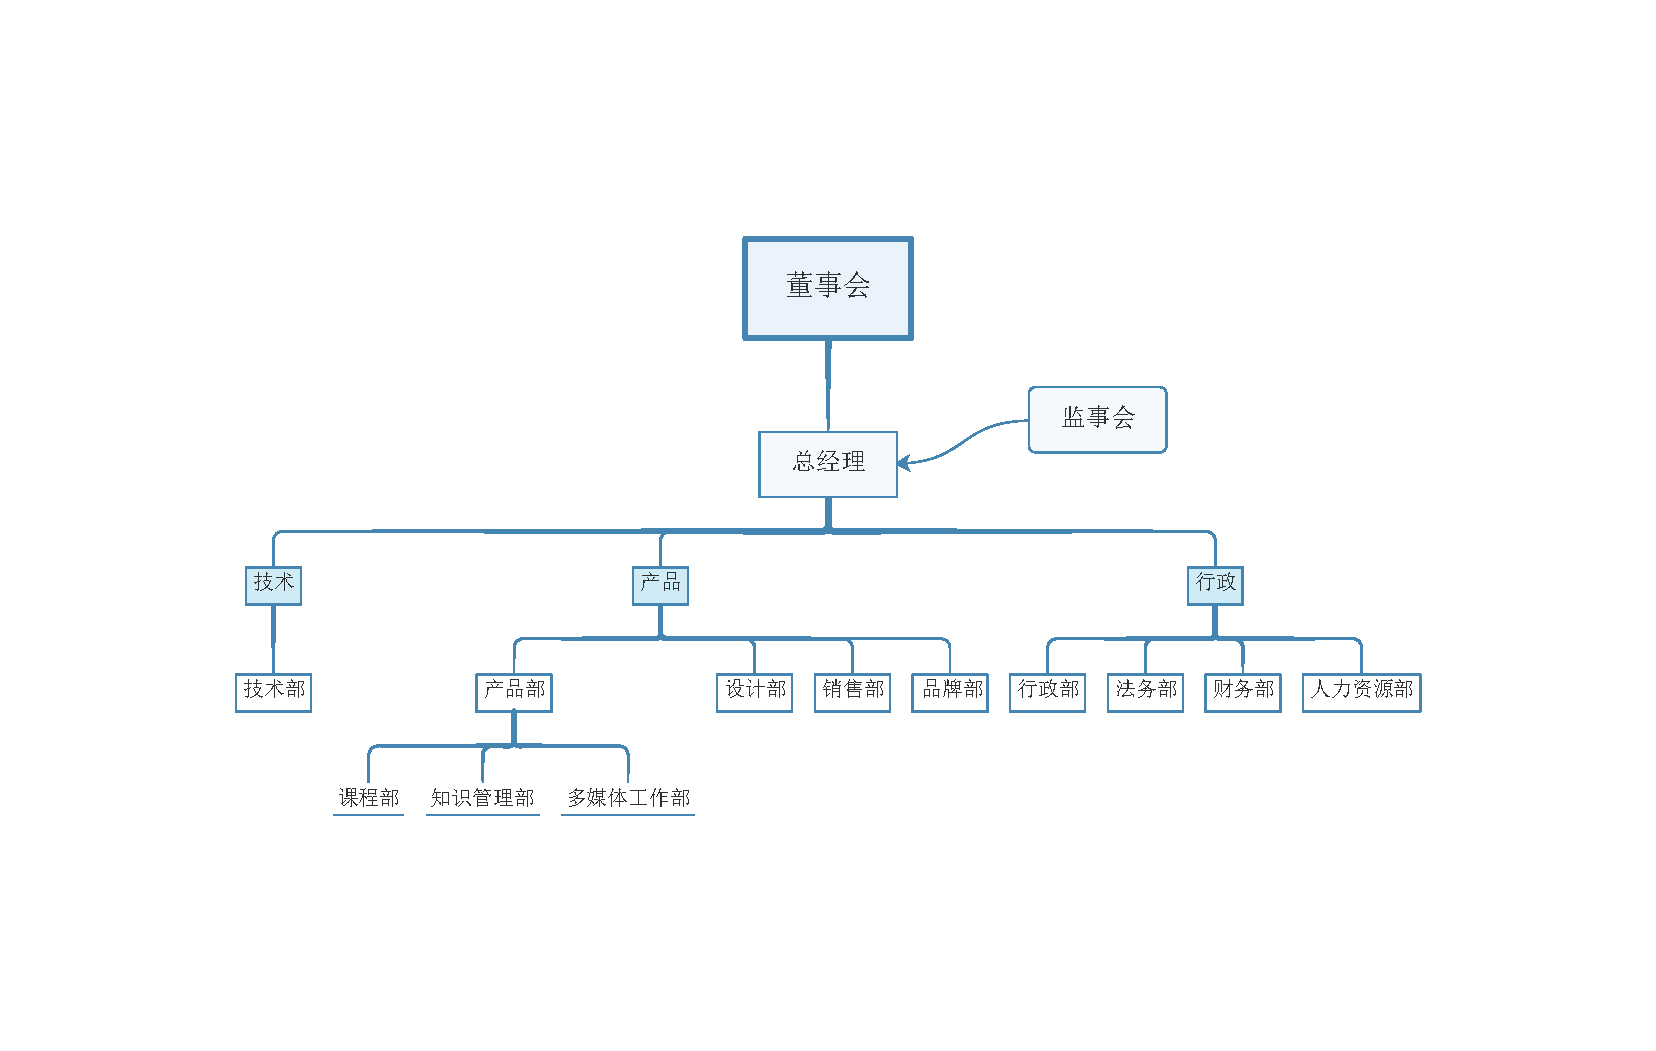
\includegraphics[width=0.9\columnwidth]{figures/management_layer}
	%  \setlength{\abovecaptionskip}{0pt}
	%  \setlength{\belowcaptionskip}{-20pt}
	\caption{公司架构图}
	\label{fg:management_layer}
\end{figure}

\subsubsection{管理层职责}\

主持公司全面工作,负责公司的全面领导和管理工作确定公司各部门分工及职权,确保公司各部门有序高效运转;

制定公司发展战略、发展计划和各项运营指标,全面把握公司的运营状况,并做出针对性调整决定;

负责把握公司业务的开展方向,与市场部、产品部、销售部等多部门协调制定公司业务暨课程内容的发展规划;

决定调整公司的组织结构、人员编制;决定公司干部的聘任、解聘、晋升和奖惩;
定期组织召开公司全体会议,检查、监督和协调各部门,各项目工作任务完成情况;

负责公司企业文化建设和员工理念、形象、素质建设,创造一流的公司品牌和公司形象;

负责公司重大项目的对外对接工作,保证公司项目运转顺利进行。

\subsection{主要业务}
\begin{itemize}
  \item 广播电视节目制作
  \item 互联网信息服务
  \item 从事互联网文化活动
  \item 出版物零售。技术开发、技术转让、技术咨询、技术服务
  \item 基础软件服务
  \item 应用软件服务
  \item 软件开发
  \item 教育咨询
  \item 组织文化艺术交流活动(不含营业性演出)
  \item 文化咨询
  \item 会议服务
  \item 承办展览展示活动
\end{itemize}


\subsection{员工组成}
课程运营人员、营销人员、系统运维人员、管理人员。

希望是全985、211高校(课程运营人员),若前期成本太高,公司可以请高校实习生,但技术人员需求专业人员或者科班出身,原因有以下三个方面:

\paragraph{节约第三方评价课程成本}\

如果公司本身就有这方面专业的高校学生,无论他学习是否好,至少他对于专业的了解是足够的,或者他直接认识专业知识非常优秀的人,或者其他同学或者师兄,师姐,老师,公司就不用再花钱去找人来评价我们不懂的课程内容了,在准确度方面也有相对较好的把握。

\paragraph{业务能力好,执行力强}\

员工组成大部分为高水平院校大学生群体,相对于其他公司人员业务能力将会更好,同时也具有更强的执行力。员工的业务能力、执行力等在一定程度上决定了公司发展的潜力,这一点对于公司的长久规划至关重要

\paragraph{人脉资源广,办事效率高}\

未来课程录制上教师选择会有许多不同需求,高水平院校大学生群体员工相对其他公司而言人脉资源更为广泛,在教师资源上将有更多选择且效率将会更高。这极大保障了公司产品的质量优势同时缩短了产品的研发周期

\subsection{公司发展目标}
公司发展理念:
\begin{figure}[H]
	\centering
	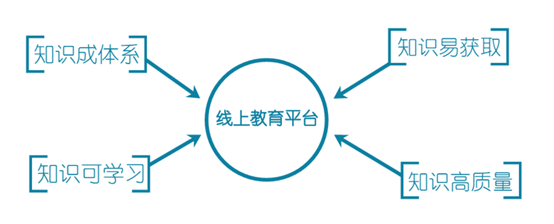
\includegraphics[width=0.9\columnwidth]{figures/company_development}%改成公司发展理念图
	%  \setlength{\abovecaptionskip}{0pt}
	%  \setlength{\belowcaptionskip}{-20pt}
	\caption{公司发展理念图}
	\label{fg:company_development}
\end{figure}

\subsubsection{近期目标}\

在公司发展前期,主要完成以下三方面任务:
\paragraph{系统研发}\

完成系统的研发工作,进行课程录制,达到一定数量后投放市场。课程需要包括视频、音频、文字这三种主要的知识载体。

\paragraph{需求调研}\

通过市场需求预调研有针对性录制迎合市场需求课程,通过校园代理或与线下机构合作的方式在短期内打开市场并实现部分盈利。课程录制的方向是:先进行市场调查,市场调查的依据是询问线下教育行业人士,然后针对性的进行课程录制,课程销售交给线下教育行业人士,获得收益分成。

\paragraph{用户积累}\

完成一定的用户资源积累,通过内容至上的核心竞争力赢得良好声誉为进一步打开市场做准备;实现部分资本回收,为下一步丰富平台资源、搭建完整课程体系做资金准备。

\begin{figure}[H]
	\centering
	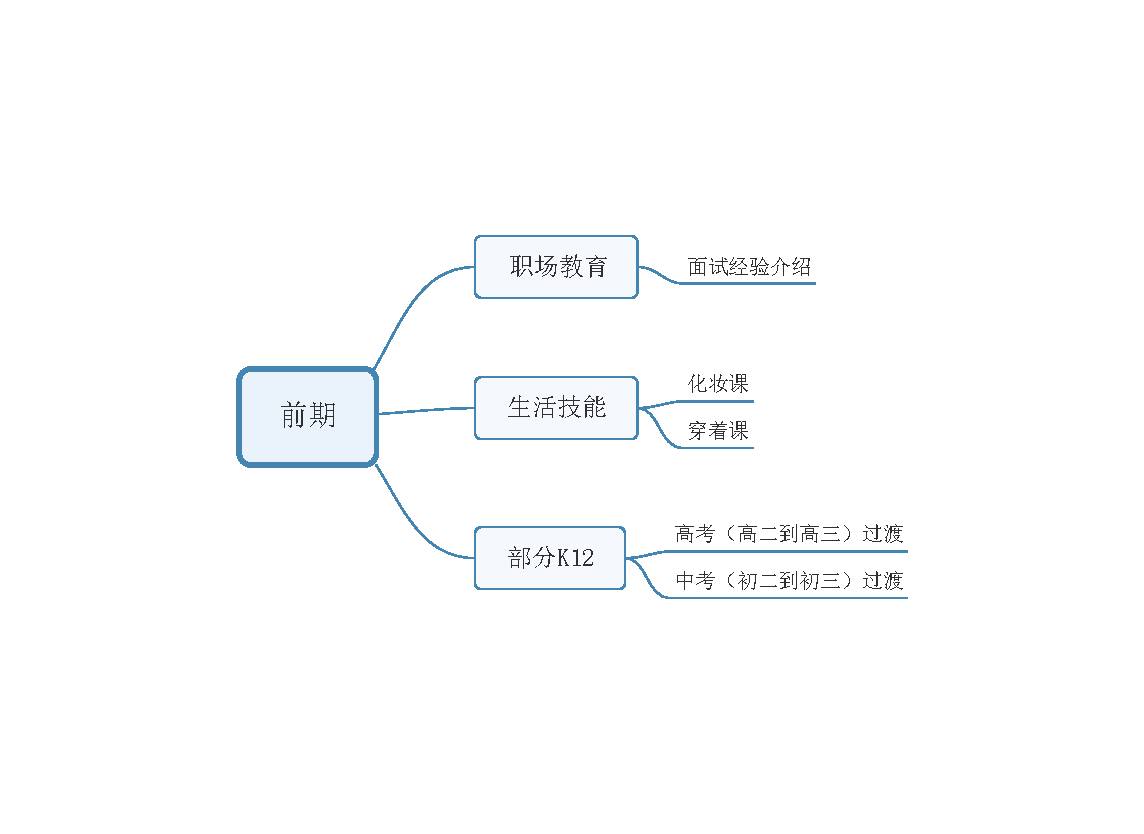
\includegraphics[width=0.9\columnwidth]{figures/prophase_development}%改图
	%  \setlength{\abovecaptionskip}{0pt}
	%  \setlength{\belowcaptionskip}{-20pt}
	\caption{前期课程发展图}
	\label{fg:prophase_development}
\end{figure}

\subsubsection{长期目标}\

在公司发展中期,主要完成以下六个方面任务:

\paragraph{增加销售人员}\

当前期盈利模式获得一定收益之后,增加销售部,销售部组成人员主要来源于社会招聘,通过市场上的有经验的销售人员,通过销售人员来留住客户。

\paragraph{课程录制转型}\

课程录制开始逐渐完善平台总体课程框架,课程录制从市场主导型转为“优先发展课程体系内市场迎合度高的产品”(市场倾向性),注重资本快速积累的同时关注长期目标实现。

\paragraph{增加品牌知名度}\

开始录制大学专业介绍类课程,同时部分课程免费开放,吸引更多用户流量以打开市场,初步拥有品牌知名度。

\paragraph{课程整合}\

对平台课程视频资源的重新整合加工,调整和优化课程内容,进一步从课程结构上提升产品质量,进一步提升产品用户活跃度与美誉度。知识管理部门初创。

\paragraph{搭建课程框架}\

涉足高等教育、从业资格教育、成人教育中部分内容,初步搭建公司全品类教育框架,在同类平台中拥有一定市场竞争力。

\paragraph{加大融资}\

进一步加大融资力度,助力公司长远发展。
\newpage
\begin{figure}[H]
	\centering
	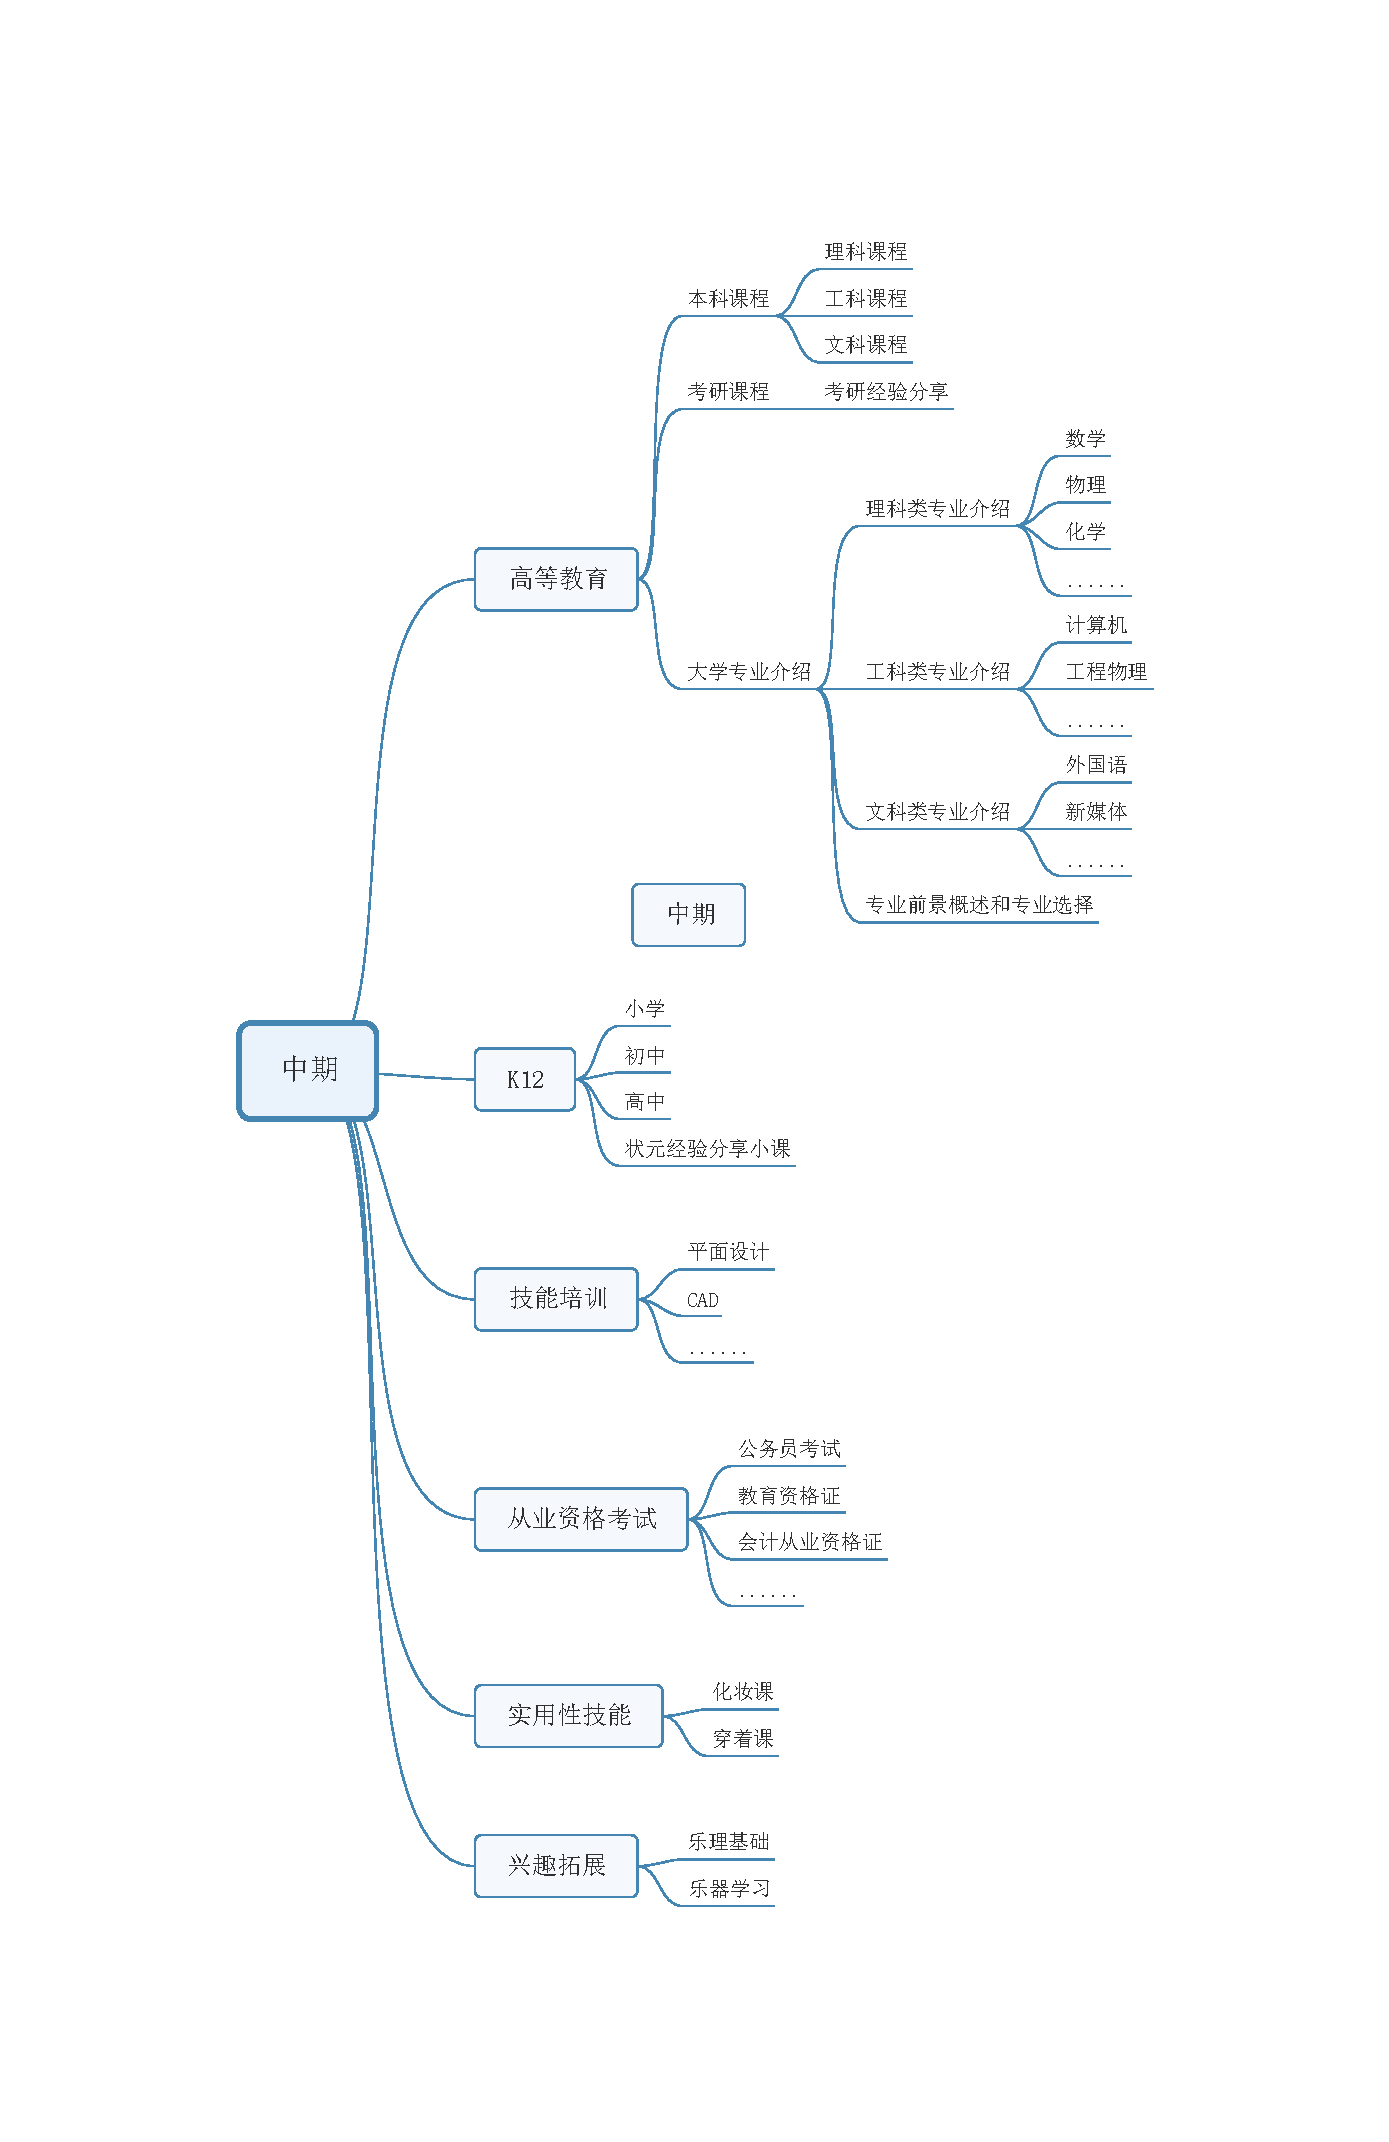
\includegraphics[width=10cm,height=17cm]{figures/mid_development}%改
	%  \setlength{\abovecaptionskip}{0pt}
	%  \setlength{\belowcaptionskip}{-20pt}
	\caption{中期课程发展图}
	\label{fg:mid_development}
\end{figure}

在公司的发展后期,我们主要完成以下任务:

\paragraph{占据较大市场份额}\

公司在在线教育行业拥有良好知名度和影响力,公司产品占据较大市场份额,资本积累达到一定高度。

\paragraph{完善课程体系}\

产品发展方向由市场倾向性变为课程体系主导型,进一步完善初始规划的课程体系,实现体系的专业性及完整性。

\paragraph{拓宽业务渠道}\

以在线教育为基础,向公司相关性产业如VR眼镜等进军,进一步拓宽业务渠道,扩大公司发展前景,增强公司生命力。

\paragraph{与政府合作}\

进军K12领域与地方政府合作,通过低价格的形式将课程卖给或者送给偏远贫困地区学生,打响平台品牌,践行公司社会责任、提升社会效益。

\paragraph{与高校合作}\

高等教育领域与高等教育院校合作,搭建高等教育知识传播平台,增强公司社会影响力,为中国人才培养提供长久而有力的支持。

\paragraph{主要盈利模式的转变}\

知识管理部门,以及公司知识创造过程的完善,以公司较完善的基础课程体系为基础,进行知识的二次加工创造,实现一个知识创造的循环。知识创造的输出以及对整个知识体系的构建,知识拓扑图的形成,对公司的产品来源、宣传上提供支持,逐渐转移主要盈利方向。

\begin{figure}[H]
	\centering
	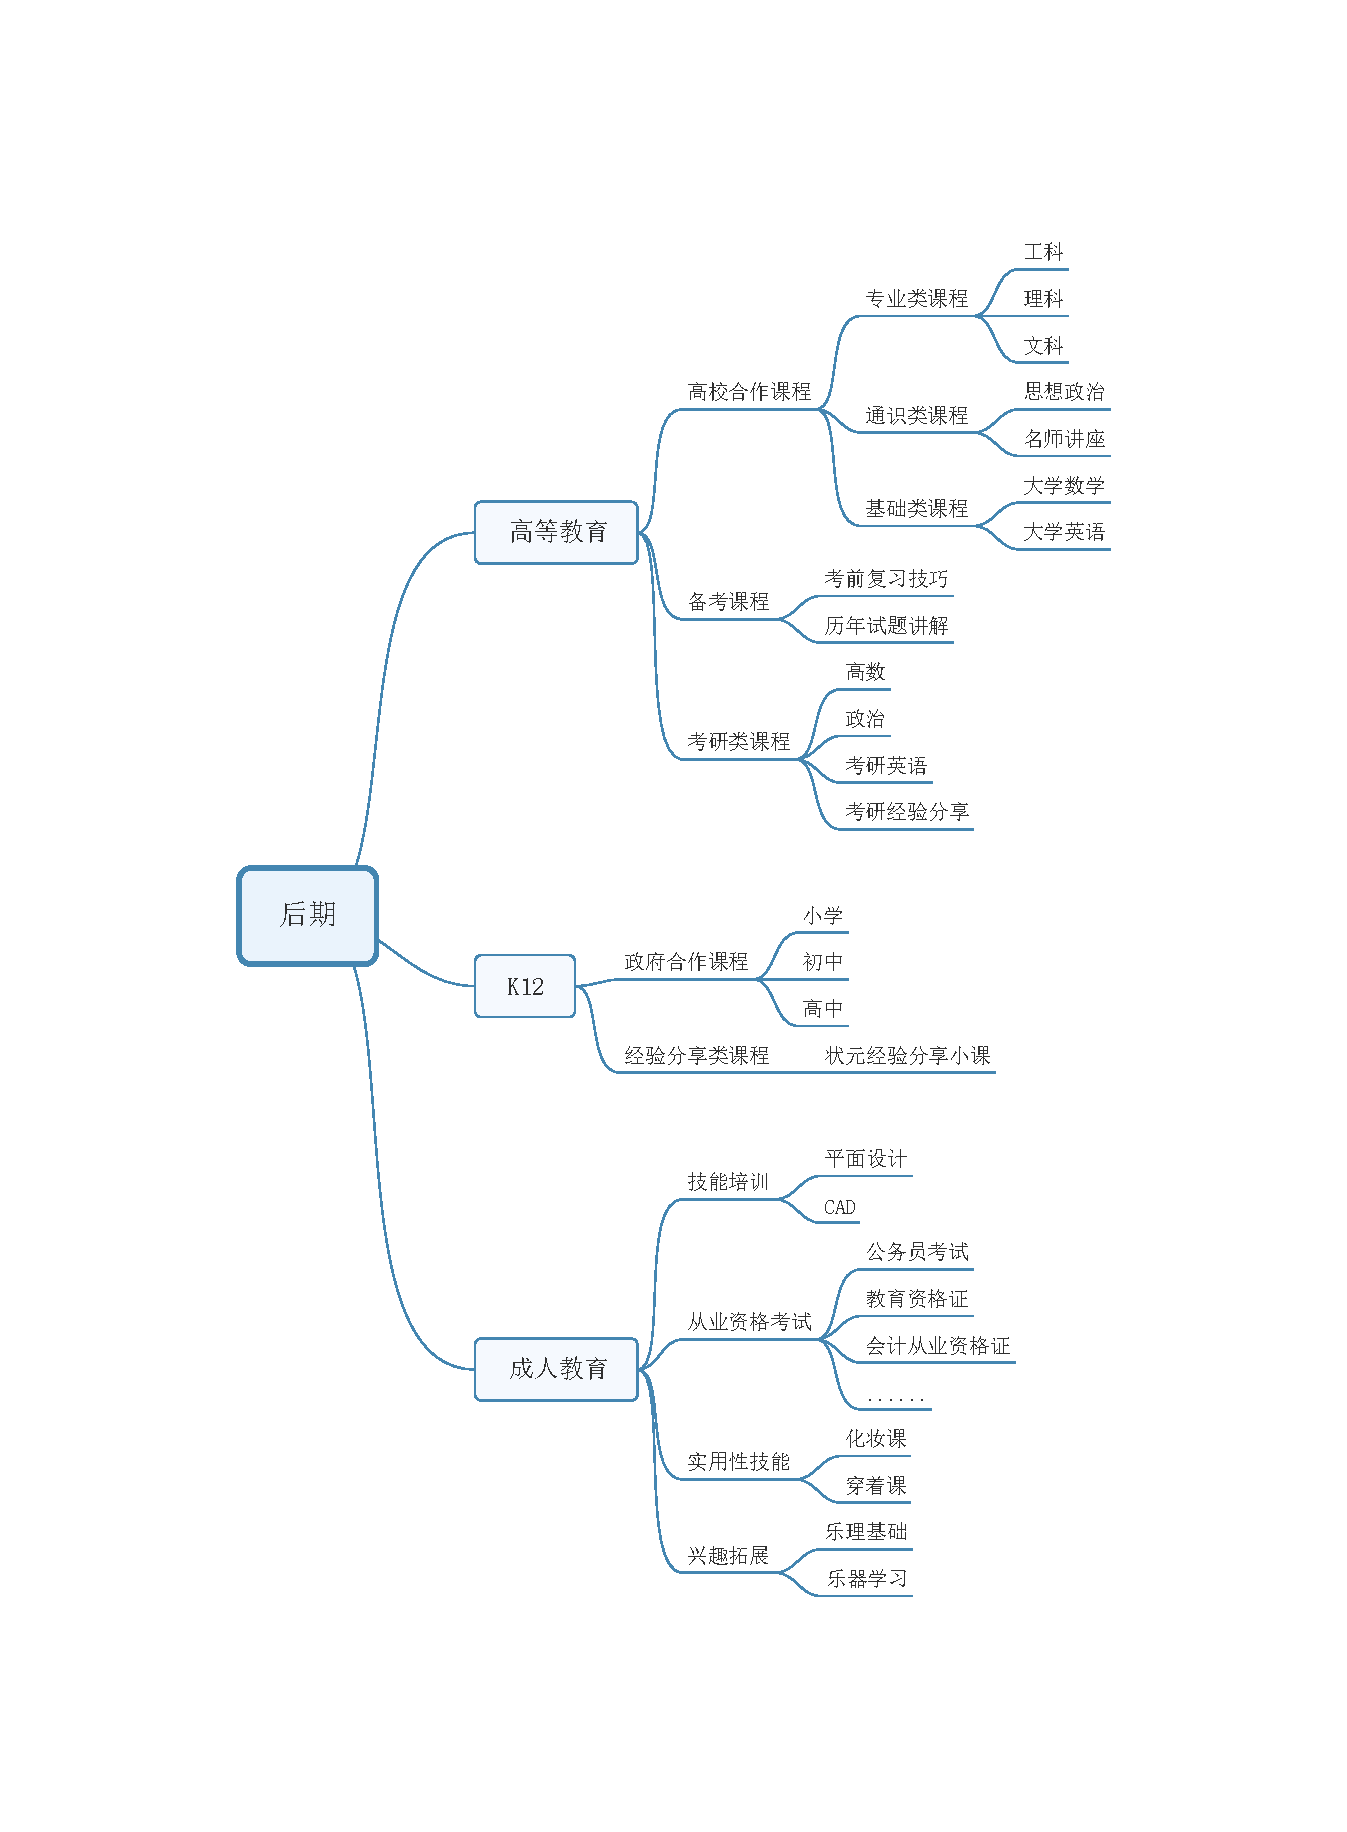
\includegraphics[width=0.9\columnwidth]{figures/aft_development}%改
	%  \setlength{\abovecaptionskip}{0pt}
	%  \setlength{\belowcaptionskip}{-20pt}
	\caption{后期课程发展图}
	\label{fg:aft_development}
\end{figure}

\subsection{三年规划五年目标}
三年内发展成为行业知名,具有一定市场影响力企业;五年内成为在线教育行业的引领者、市场规则的制定者,在追求经济效益的同时践行公司的社会责任。

\subsection{公司文化}
做一个服务用户的合作者,为有志青年提供知识改变命运的途径;

做一个理想的知识获取平台,为人才培养提供支持;

做网络知识领域的一面旗帜,为知识创新提供长远的推动力。

来一课,选择适合你的一课

这一课,不错过。














